\documentclass[12pt]{article}
\usepackage[a4paper,left=27mm,right=27mm,top=25mm,bottom=20mm]{geometry}
\usepackage[space]{ctex}
\usepackage{graphicx}
\usepackage{float}
\usepackage{subfigure}
\usepackage{amsmath}
\title{\LARGE\textbf{Workpaper}}
\author{SA21010060 周俊亦}
\date{}

\begin{document}
	\maketitle
	\renewcommand{\abstractname}{Abstract}
	\begin{abstract}
		本报告复现了论文\textsl{Color Transfer between Images}中的工作。该算法将图像映射到空间进行伸缩变换,得到改变图像的色调的效果。
	\end{abstract}
	
	\section{算法原理}
		\subsection{算法介绍}
		彩色图像由一个个像素构成,操纵图像的色调,势必将对图像的一个个像素进行操作。图像的色彩空间是一堆三维点簇,一个显而易见的想法是在RGB的三维点空间进行一系列变换。然而,RGB空间的点与点之间有很强的相关性。
		
		\begin{figure}[htbp]
			\centering
			\subfigure[RGB空间]{
				\begin{minipage}[t]{0.5\linewidth}
					\centering
					\includegraphics[width=2.5in]{./1.jpg}
					%\caption{fig1}
				\end{minipage}%
			}%
			\subfigure[$ l\alpha \beta $空间]{
				\begin{minipage}[t]{0.5\linewidth}
					\centering
					\includegraphics[width=2.5in]{./2.jpg}
					%\caption{fig2}
				\end{minipage}%
			}
			\centering
			\caption{RGB空间与$ l\alpha \beta $空间的散点图}
		\end{figure}
		
		如图1(a)所示,RGB空间的图像点云是一个三维椭球,在RGB点云上进行变换很难达到良好的效果。因此,本文作者将相关性较强的RGB空间点云变换到相关性较弱的空间点云(如图1(b)所示,空间的图像点云近似为直线,有较弱的相关性),在此基础上进行点云变换,完成图像的色调转换。
		
		\newpage
		\subsection{原理}
		算法的输入为:原始图像source、色调样例target; 算法输出为result。即算法将target的色调映射到source上,使source改变色调。\\
		
		图像转换过程总体分为两个步骤:\\ 
		
		\textbf{第一步:}通过:
		\begin{equation*}
			{\left[ \begin{array}{ccc}
					L\\
					M\\
					S
				\end{array} 
				\right ]}={
				\left[ \begin{array}{ccc}
					0.3811 & 0.5783 & 0.0402\\
					0.1967& 0.7244 & 0.0782\\
					0.0241 & 0.1288 & 0.8444
				\end{array} 
				\right ]}{\left[ \begin{array}{ccc}
					R\\
					G\\
					B
				\end{array} 
				\right ]} 
		\end{equation*} 
		\begin{align*}
			\textbf{L} &= log(L) \\
			\textbf{M} &= log(M) \\
			\textbf{S} &= log(S)
		\end{align*}
	\begin{equation*}
		{\left[ \begin{array}{ccc}
				l\\
				\alpha\\
				\beta
			\end{array} 
			\right ]}={
			\left[ \begin{array}{ccc}
				\frac{1}{\sqrt{3}} & 0 & 0\\
				0& \frac{1}{\sqrt{6}} & 0\\
				0 & 0 & \frac{1}{\sqrt{2}}
			\end{array} 
			\right ]}
		{
			\left[ \begin{array}{ccc}
				1 & 1 & 1\\
				1& 1 & -2\\
				1 & -1 & 0
			\end{array} 
			\right ]}{\left[ \begin{array}{ccc}
				\textbf{L}\\
				\textbf{M}\\
				\textbf{S}
			\end{array} 
			\right ]} 
	\end{equation*} 
	将source 和 target 转换到$ l\alpha\beta $空间,随后计算source和target的均值和标准差$ \mu_s, \sigma_s, \mu_t, \sigma_t $。\\ 
	
	\textbf{第二步:}对source的每一个像素s,通过:
	\begin{equation*}
		s^{\prime} = \frac{\sigma_t}{\sigma_s} (s - \mu_s) + \mu_t
	\end{equation*}
    作变换。

	\section{实验分析}
	在i5-8300H CPU @ 2.30GHz 下,使用 opencv 3.4.15进行算法验证。表1列出了部分样例算法用时。由于除了像素计算工作,没有别的数据处理工作,所以算法的时间复杂度是$ O(n\times m)$。一般大小的图片都可以在1s以内换完毕。之后列出了部分测试用例。
	
	\begin{table}[H]
		\centering
		\caption{算法效率}
		\begin{tabular}{|c|c|c|c|c|}
			\hline
			source      & target      & read time(s) & algorithm(s) & total(s)  \\ \hline
			270 x 180   & 240 x 180   & 0.0014265    & 0.0243411    & 0.0257676 \\ \hline
			1024 x 640  & 1440 x 900  & 0.0285507    & 0.407667     & 0.436218  \\ \hline
			1920 x 1200 & 1080 x 1080 & 0.0600101    & 0.87057      & 0.93058   \\ \hline
		\end{tabular}
	\end{table}
	
	\begin{figure}[htbp]
		\centering
		\subfigure[source(270x180)]{
			\begin{minipage}[t]{0.3\linewidth}
				\centering
				\includegraphics[width=1.7in]{../1.jpg}
				%\caption{fig1}
			\end{minipage}%
		}%
		\subfigure[target(240x180)]{
			\begin{minipage}[t]{0.3\linewidth}
				\centering
				\includegraphics[width=1.7in]{../2.jpg}
				%\caption{fig2}
			\end{minipage}%
		}
	\subfigure[result]{
		\begin{minipage}[t]{0.3\linewidth}
			\centering
			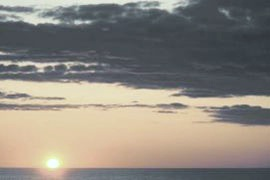
\includegraphics[width=1.7in]{./result1.jpg}
			%\caption{fig2}
		\end{minipage}%
	}
		\centering
		\caption{Example-1}
	\end{figure}

	\begin{figure}[htb]
		\centering
		\subfigure[source(240x180)]{
			\begin{minipage}[t]{0.3\linewidth}
				\centering
				\includegraphics[width=1.7in]{../2.jpg}
				%\caption{fig1}
			\end{minipage}%
		}%
		\subfigure[target(270x180)]{
			\begin{minipage}[t]{0.3\linewidth}
				\centering
				\includegraphics[width=1.7in]{../1.jpg}
				%\caption{fig2}
			\end{minipage}%
		}
		\subfigure[result]{
			\begin{minipage}[t]{0.3\linewidth}
				\centering
				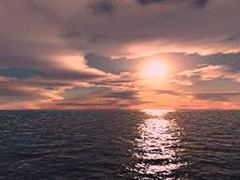
\includegraphics[width=1.7in]{./result2.jpg}
				%\caption{fig2}
			\end{minipage}%
		}
		\centering
		\caption{Example-2}
	\end{figure}

	\begin{figure}[H]
		\centering
		\subfigure[source(1024x640)]{
			\begin{minipage}[t]{0.3\linewidth}
				\centering
				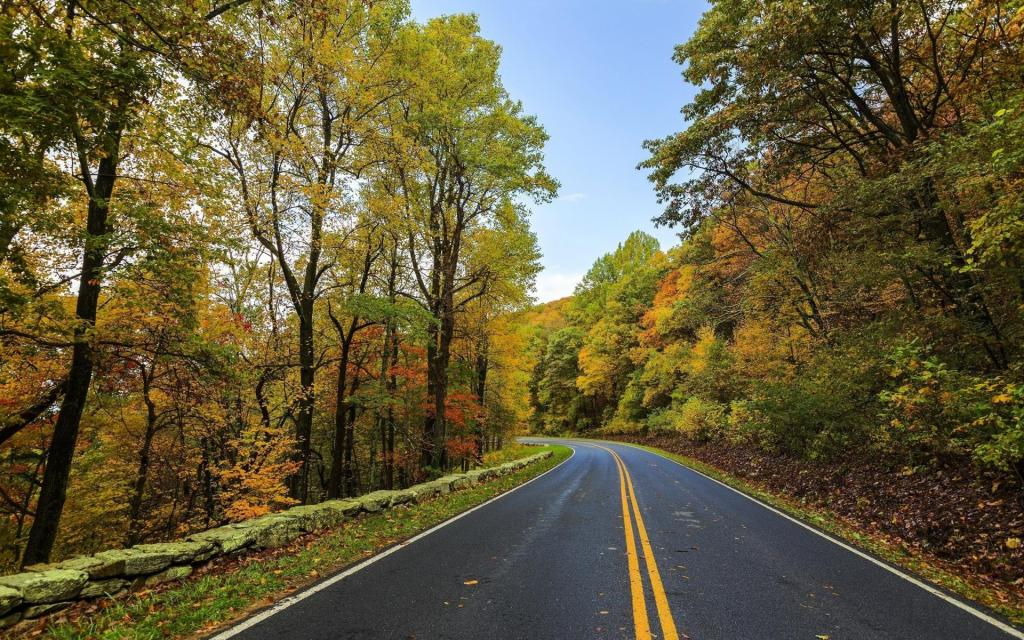
\includegraphics[width=1.7in]{../8.jpg}
				%\caption{fig1}
			\end{minipage}%
		}%
		\subfigure[target(1440x900)]{
			\begin{minipage}[t]{0.3\linewidth}
				\centering
				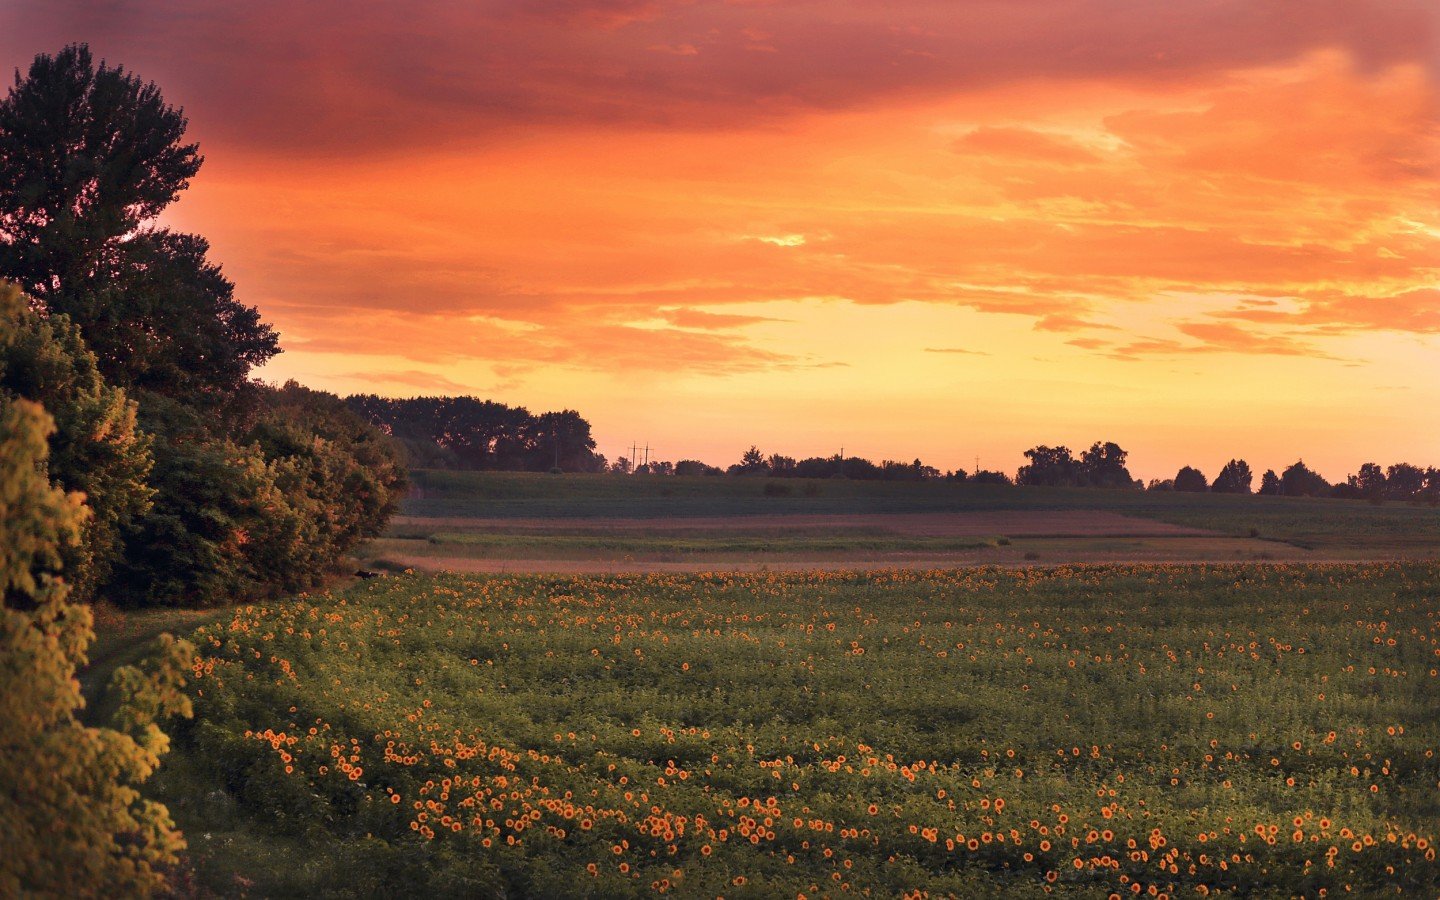
\includegraphics[width=1.7in]{../9.jpeg}
				%\caption{fig2}
			\end{minipage}%
		}
		\subfigure[result]{
			\begin{minipage}[t]{0.3\linewidth}
				\centering
				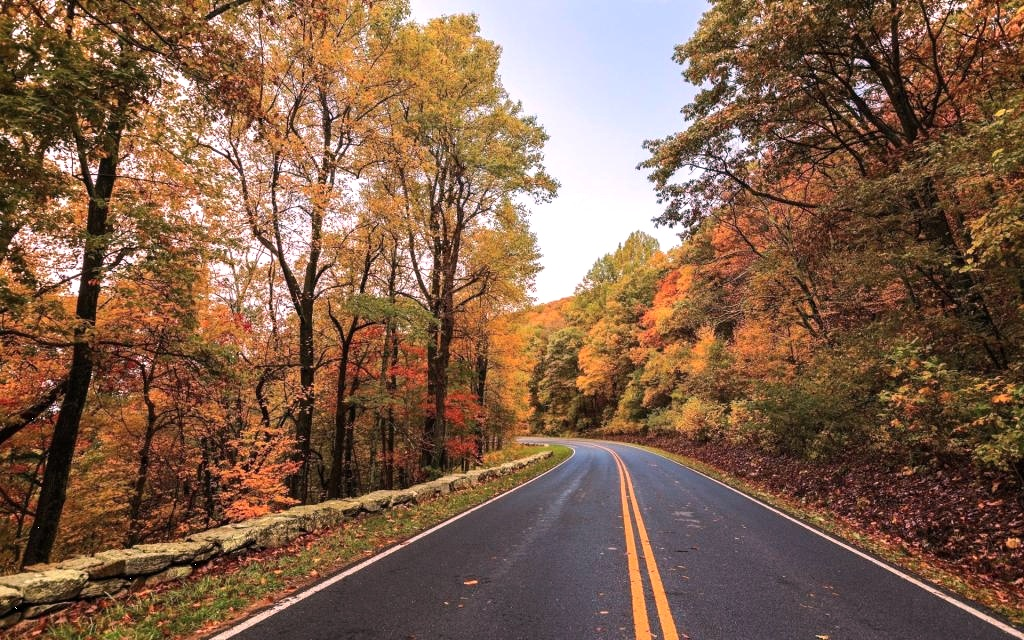
\includegraphics[width=1.7in]{./result4.jpg}
				%\caption{fig2}
			\end{minipage}%
		}
		\centering
		\caption{Example-3}
	\end{figure}

	\begin{figure}[htbp]
		\centering
		\subfigure[source(1920x1200)]{
			\begin{minipage}[t]{0.3\linewidth}
				\centering
				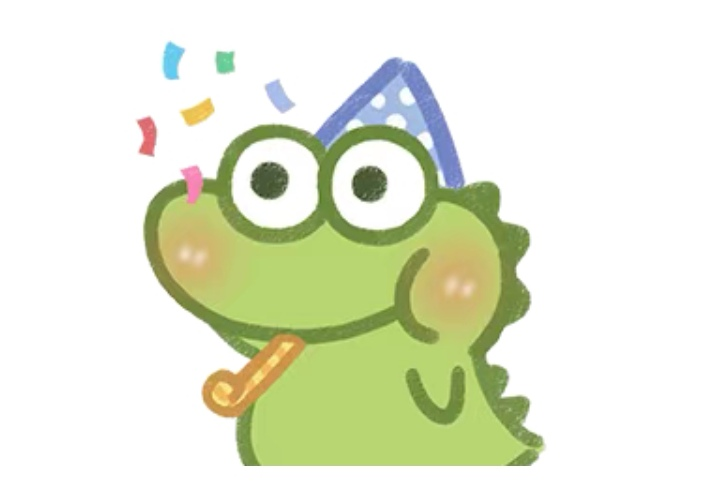
\includegraphics[width=1.7in]{../5.jpg}
				%\caption{fig1}
			\end{minipage}%
		}%
		\subfigure[target(1080x1080)]{
			\begin{minipage}[t]{0.3\linewidth}
				\centering
				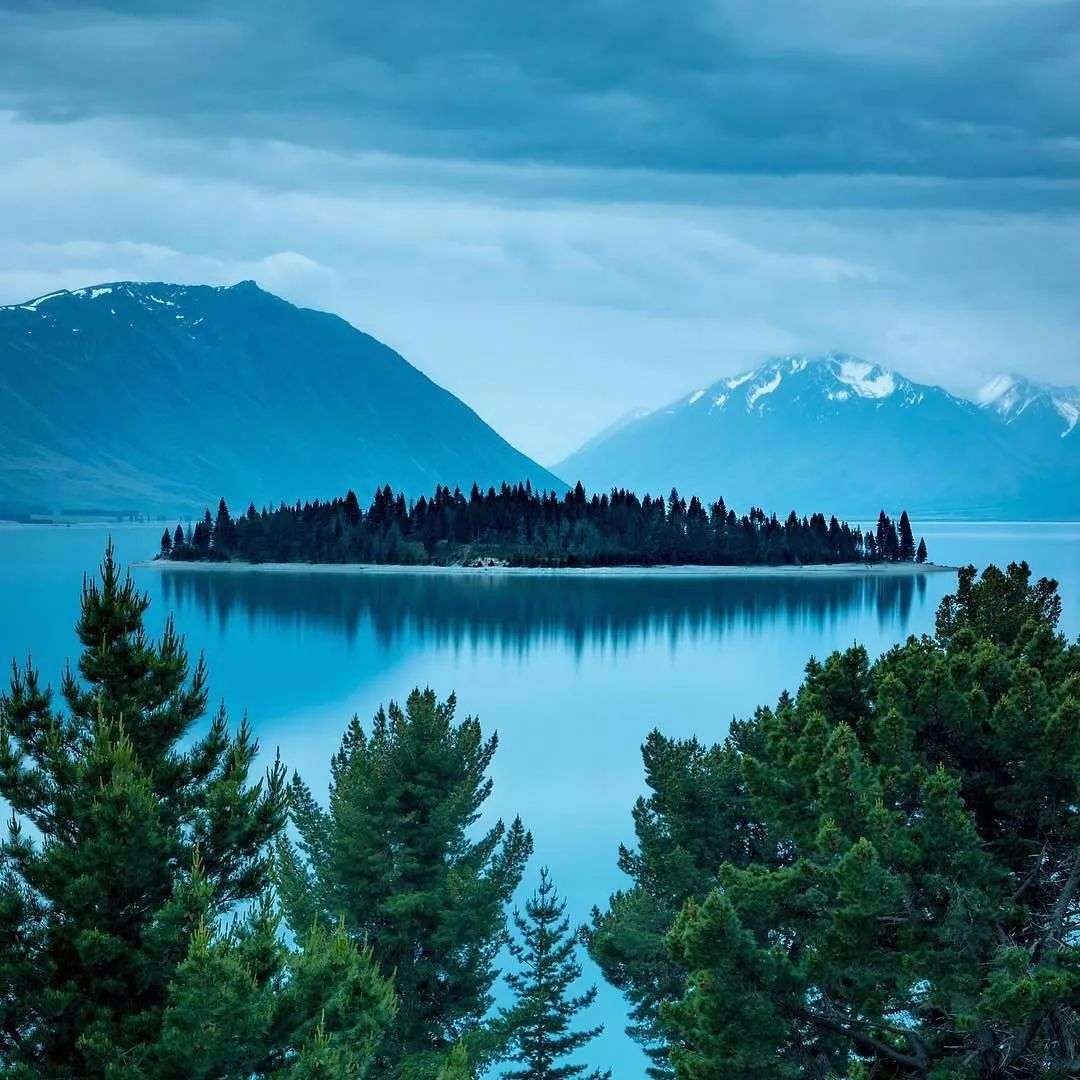
\includegraphics[width=1.4in]{../6.jpg}
				%\caption{fig2}
			\end{minipage}%
		}
		\subfigure[result]{
			\begin{minipage}[t]{0.3\linewidth}
				\centering
				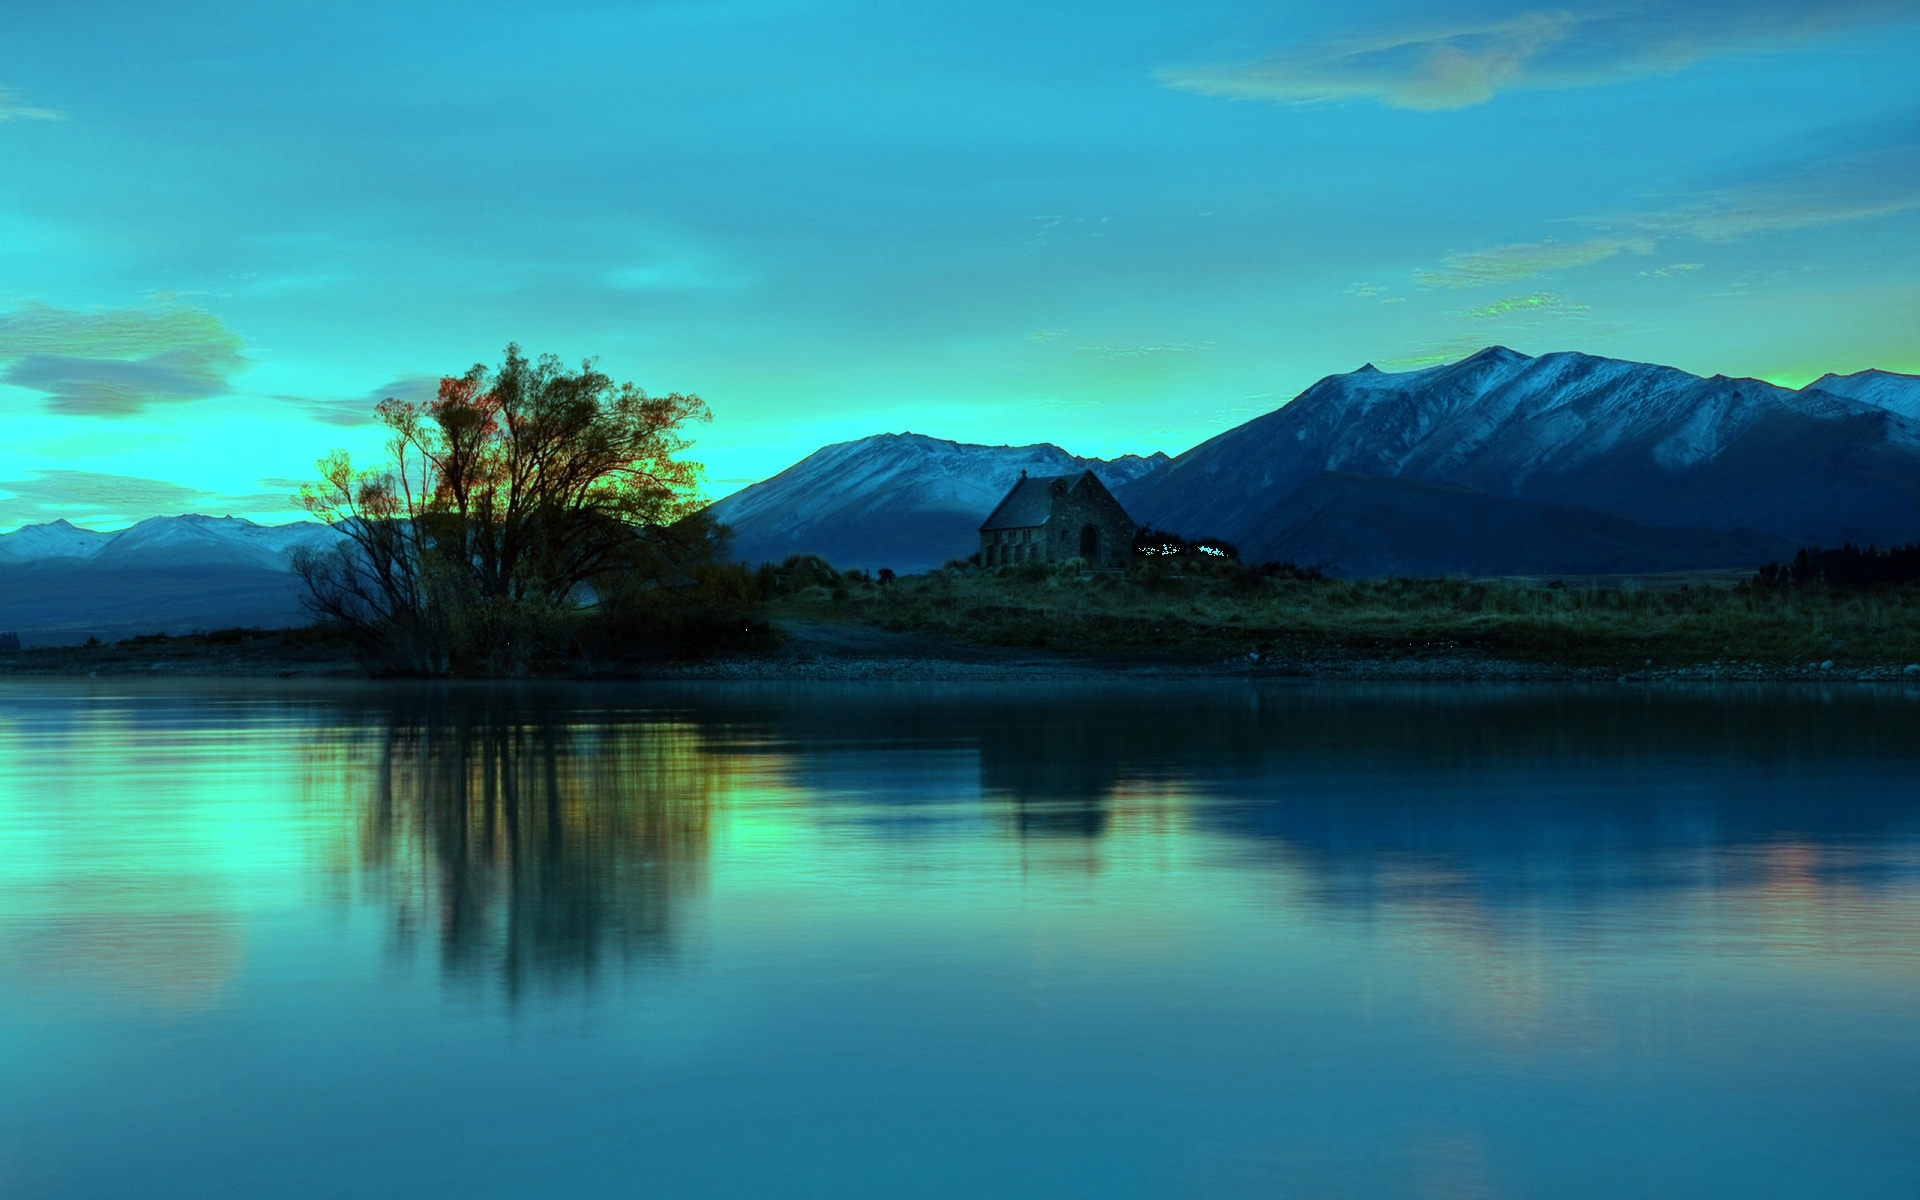
\includegraphics[width=1.7in]{./result3.jpg}
				%\caption{fig2}
			\end{minipage}%
		}
		\centering
		\caption{Example-4}
	\end{figure}
	
	\begin{figure}[H]
		\centering
		\subfigure[source]{
			\begin{minipage}[t]{0.3\linewidth}
				\centering
				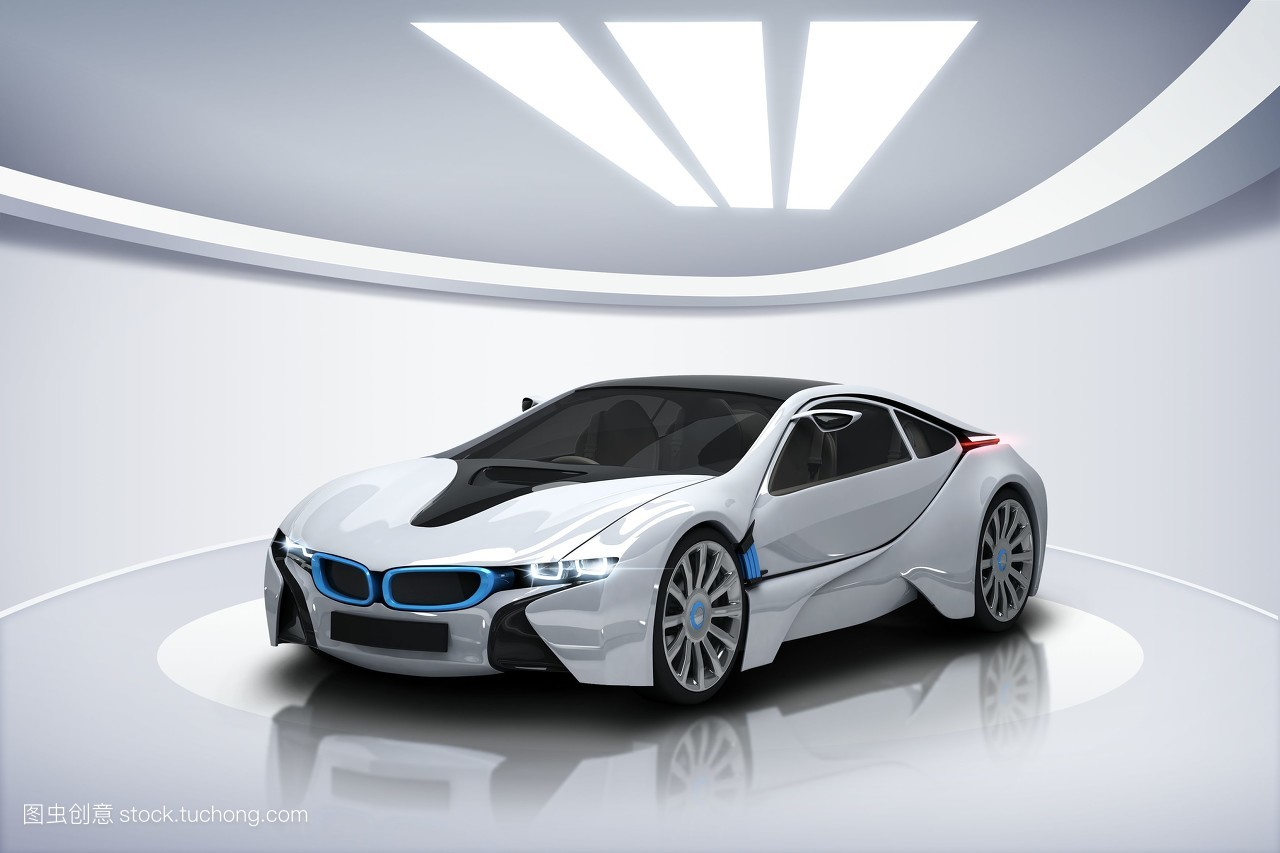
\includegraphics[width=1.7in]{../11.jpg}
				%\caption{fig1}
			\end{minipage}%
		}%
		\subfigure[target]{
			\begin{minipage}[t]{0.3\linewidth}
				\centering
				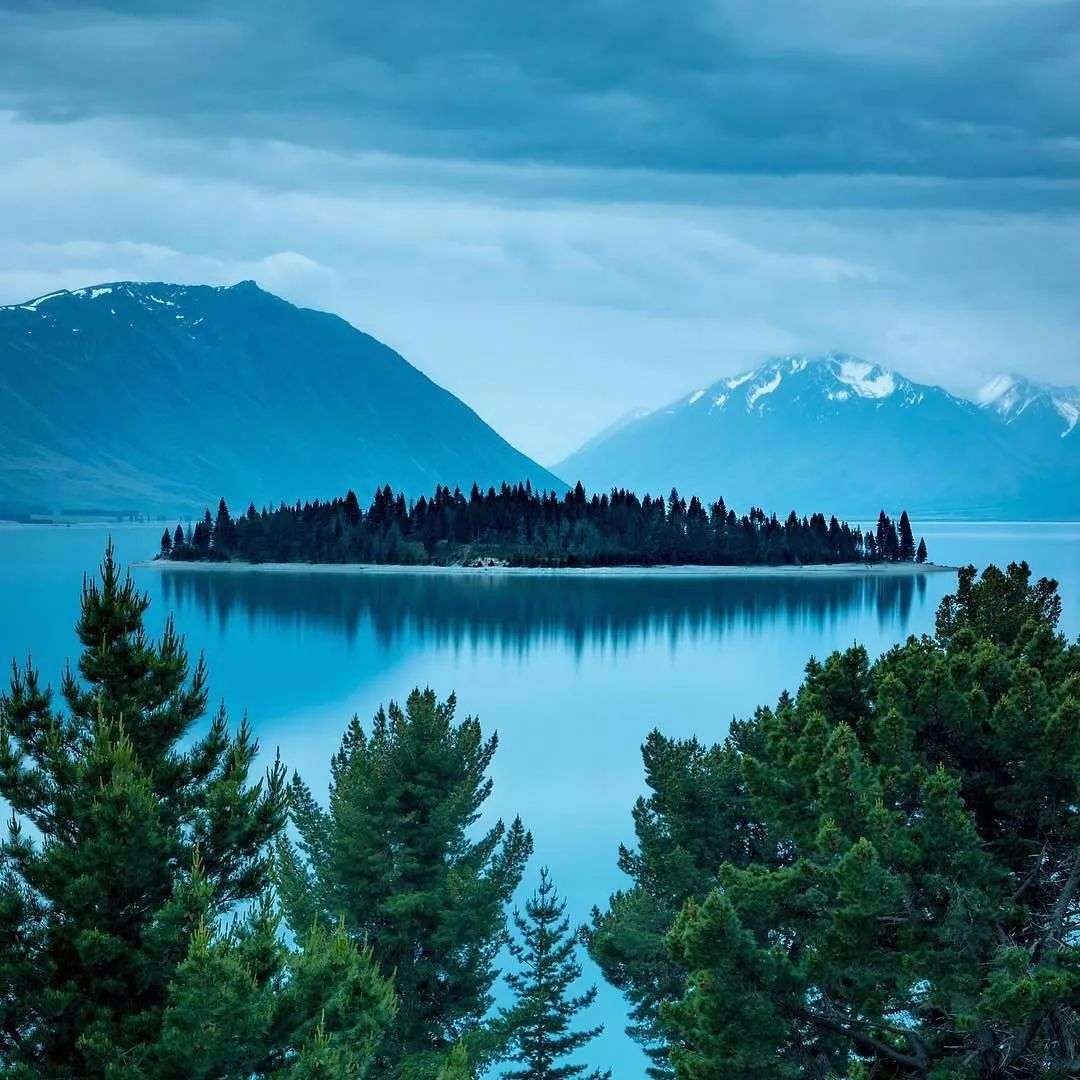
\includegraphics[width=1.4in]{../6.jpg}
				%\caption{fig2}
			\end{minipage}%
		}
		\subfigure[result]{
			\begin{minipage}[t]{0.3\linewidth}
				\centering
				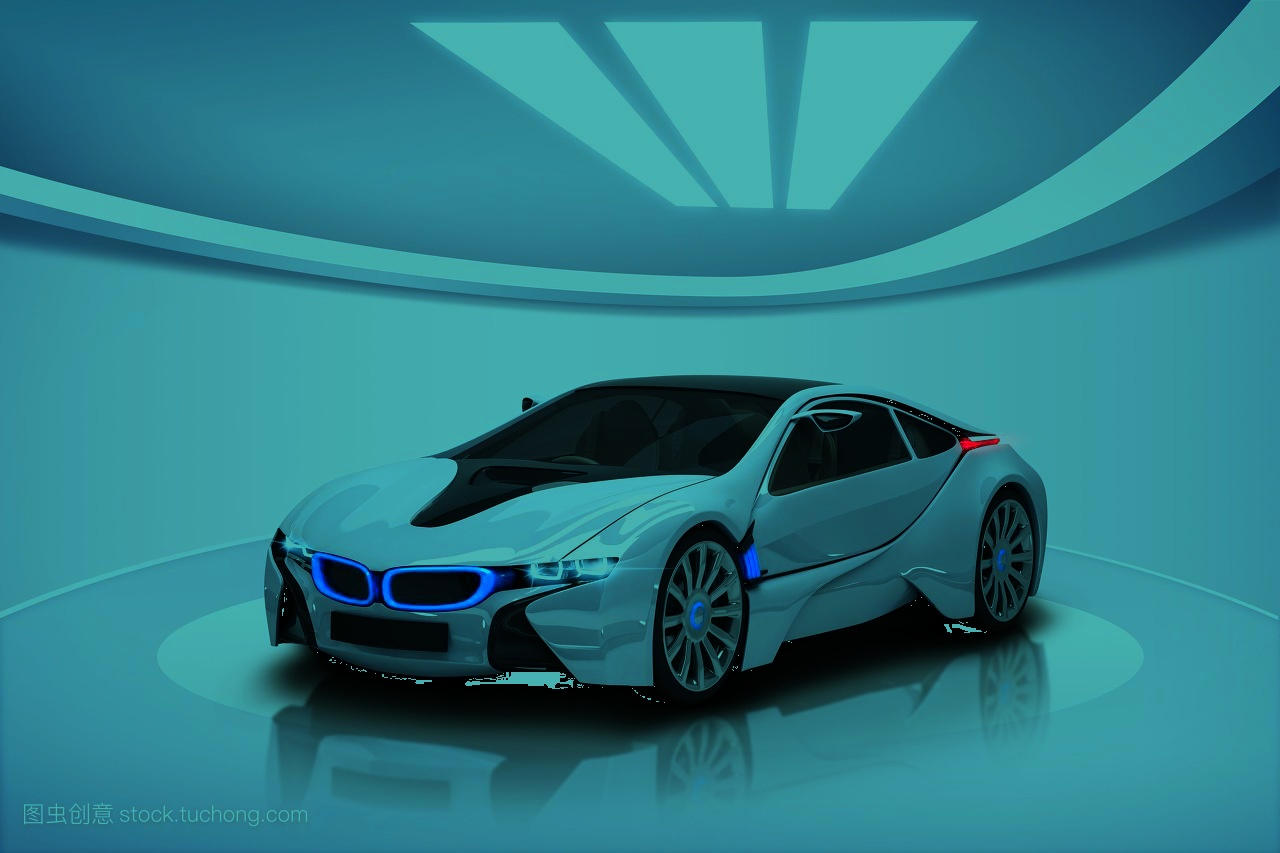
\includegraphics[width=1.7in]{./result5.jpg}
				%\caption{fig2}
			\end{minipage}%
		}
		\centering
		\caption{Example-5(语义不一致)}
	\end{figure}
	
	\begin{figure}[H]
		\centering
		\subfigure[source]{
			\begin{minipage}[t]{0.3\linewidth}
				\centering
				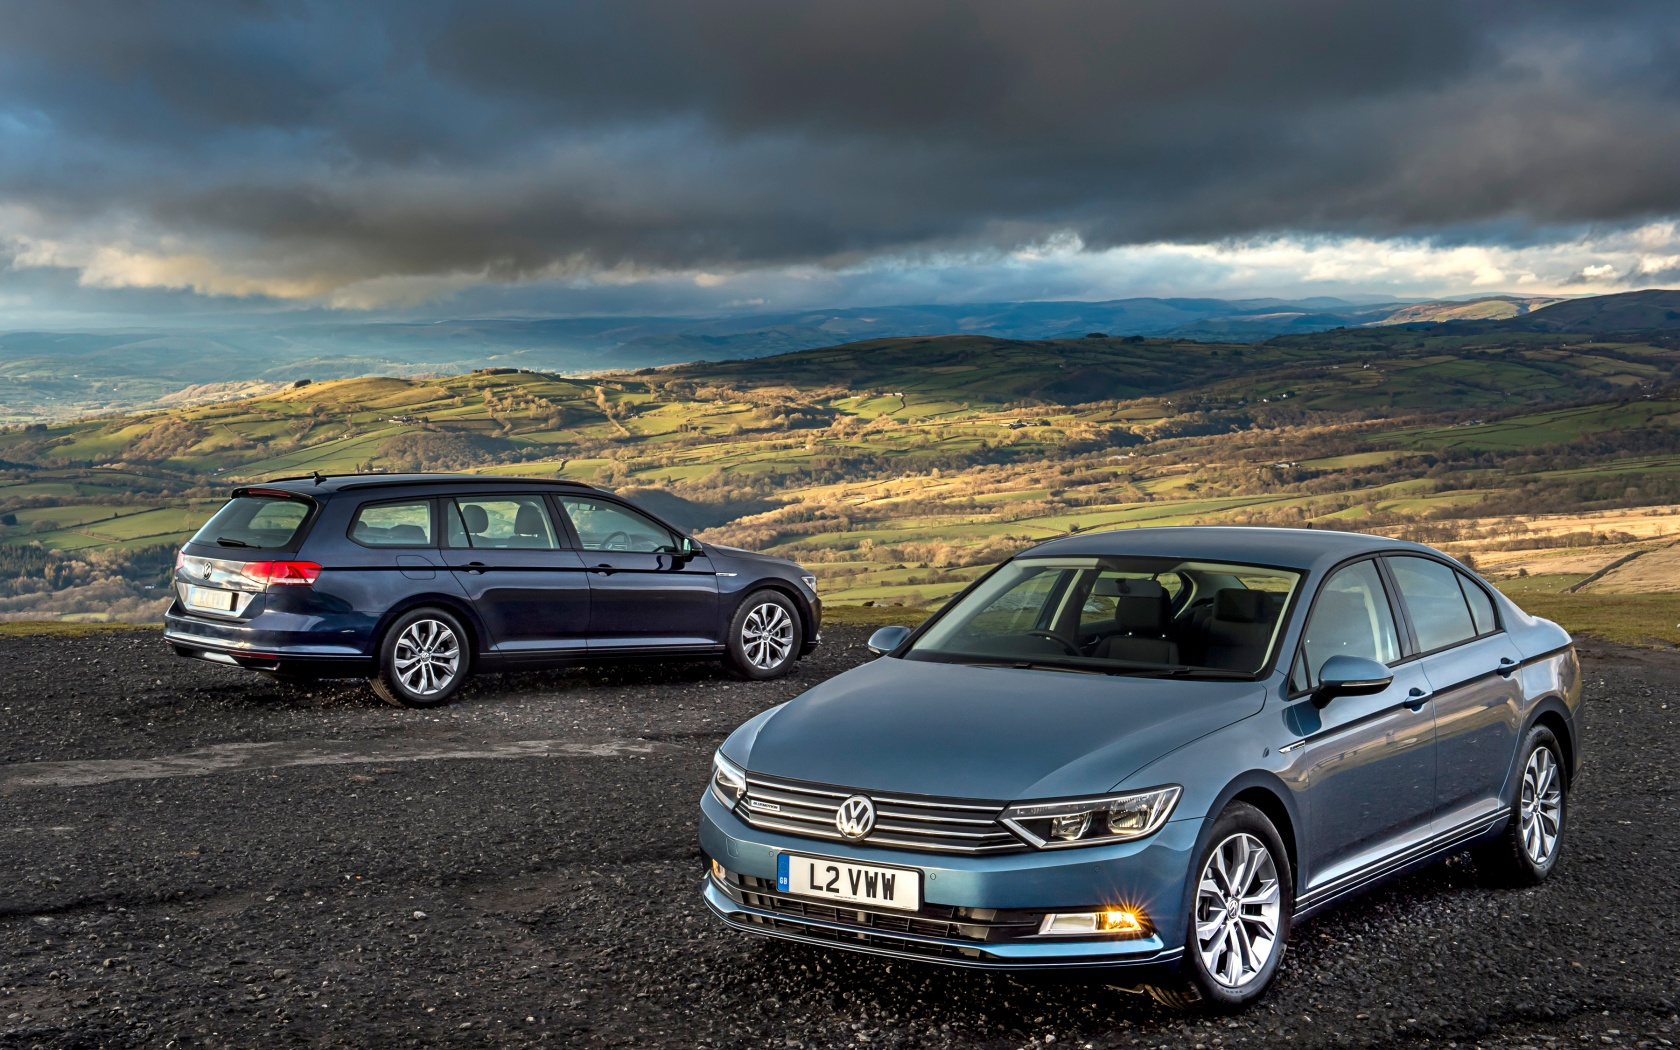
\includegraphics[width=1.7in]{../10.jpeg}
				%\caption{fig1}
			\end{minipage}%
		}%
		\subfigure[target]{
			\begin{minipage}[t]{0.3\linewidth}
				\centering
				\includegraphics[width=1.4in]{../1.jpg}
				%\caption{fig2}
			\end{minipage}%
		}
		\subfigure[result]{
			\begin{minipage}[t]{0.3\linewidth}
				\centering
				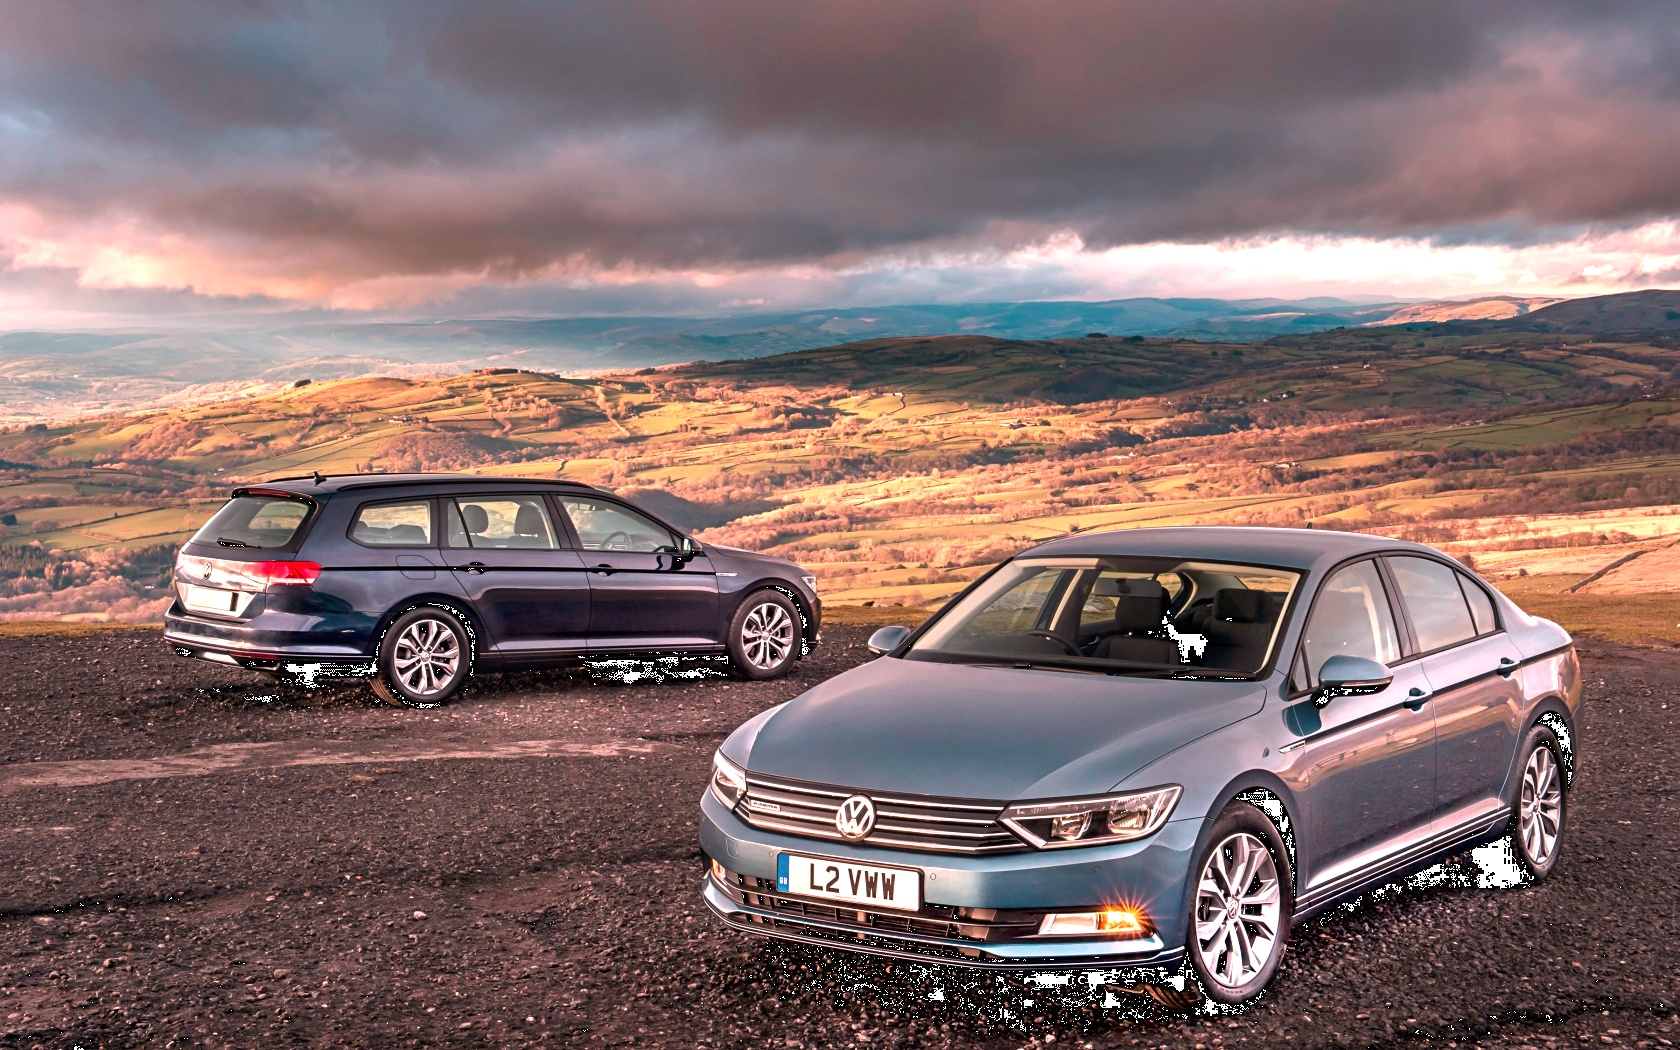
\includegraphics[width=1.7in]{./result6.jpg}
				%\caption{fig2}
			\end{minipage}%
		}
		\centering
		\caption{Example-6(语义不一致)}
	\end{figure}
	通过以上样例发现,在图片语义类似的情况下,主观评测测试用例效果良好。在语义不一致的情况下,整体色调转换效果同样良好,但是原图较暗的区域转化后存在白点。
	
	\section{实验总结}
	本次实验复现了论文中的算法,对算法的理解得到了提升。文中对图像的处理只是简单的利用了均值和方差,利用主成分分析或许能得到更好的效果。
	
	\begin{thebibliography}{99}
		\bibitem{1} Color Transfer: E. Reinhard et al. Color Transfer between Images. IEEE CGA, 2001.
	\end{thebibliography}
\end{document}

